% **************************************************************************************************
% **************************************************************************************************
\newsection{Deep Learning}{fundamentals:deep-learning}
Although the first artificial neural networks were implemented in the 1950s, the practical use of these small networks was limited. It was not until half a century later, when neural networks became significantly larger, that the first major successes could be celebrated. In the mid 2010s, \glspl{dnn} like the \textit{AlexNet}~\cite{krizhevsky2012imagenet} started to win \gls{cv} competitions. These \glspl{dnn}, mainly \glspl{cnn}, try to get rid of the traditional two-step architecture -- feature engineering followed by a simple machine learning algorithm. Instead, \glspl{dnn} are trained to learn suitable feature representations by themself (see Fig.~\ref{fig:ml-vs-deeplearning}). Usually, the first layers detect simple patterns, such as edges and corners in images, in the input data. The following layers utilize these features to learn more complex concepts like object parts.\\
\figc{width=0.6\textwidth}{\pwd/figs/classical_ml_vs_deeplearning}{The transition from \enquote{classical} machine learning to deep learning.}{ml-vs-deeplearning}

Two main factors contributed to the breakthrough of deep learning: the availability of large datasets and the increase in processing power through the use of \glspl{gpu}. Since \glspl{dnn} have large numbers of learnable parameters, huge amounts of training data are needed to avoid overfitting. This is especially true if models are trained from scratch with randomly initialized weights. Until recently, available data was not sufficient to train models with millions of parameters. In 2009, \textit{ImageNet}~\cite{deng2009imagenet} -- the first large-scale database for \gls{cv} with over 14 million images -- was released. Unfortunately, for most of the tasks in \gls{mir}, there are still no such datasets. The authors of~\cite[p.~19]{goodfellow2016book} claim that \enquote{\dots the amount of skill required reduces as the amount of training data increases.} To compensate for the lack of data, it is common to extend datasets by artificially creating new samples from the original ones, a practice known as \textit{data augmentation}. \textit{Transfer learning}, the reuse of a model trained for a particular task for another similar task, is also a popular technique, when data is scarce. Both, data augmentation and transfer learning, have been extensively applied in the course of this work and are explained in detail in Chapter~\ref{chp:method}. As mentioned earlier, besides massive datasets, a lot of computing power is essential for deep learning. For this reason, in 2007, \textit{NVIDIA} released the \textit{CUDA}~\cite{nickolls2008cuda} API which allows programmers to use \glspl{gpu} for general purpose processing. As the name suggests, \glspl{gpu} have originally been designed for graphics applications. However, their capability to perform many computations in parallel makes them highly suitable for matrix multiplications, which are extensively involved in training of \glspl{dnn}. Luckily, deep learning frameworks like \textit{PyTorch}~\cite{paszke2019pytorch} natively support \textit{CUDA}, so researchers can focus on their scientific work without having to dive deep into parallel computing.

\newsubsection{Convolutional Neural Networks (CNNs)}{fundamentals:deep-learning:cnn}
Out of all the variants of \glspl{dnn} available today, \glspl{cnn} are probably the most popular architecture. Nevertheless, this hype around \glspl{cnn} is well justified, considering their immense success in \gls{cv} competitions such as the \textit{ImageNet Large Scale Visual Recognition Challenge (ILSVRC)} in recent years. However, the application of \glspl{cnn} is not limited to the distinction of cats and dogs. \Glspl{cnn} also received much attention in \gls{mir} and especially music classification tasks like genre, mood and instrument classification~\cite{nam2018deep}.

\newsubsubsection{Why CNNs?}{fundamentals:deep-learning:cnn:why}
\Glspl{cnn} were originally developed for pattern recognition in images. Yet these models can basically be deployed for any data exhibiting a spatial structure, including 1D time series such as digital audio signals and 2D time-frequency representations like spectrograms. Conventional feed-forward neural networks are prone to overfitting due to their large number of parameters~\cite{oshea2015introToCNN}. Consider a color input image of size $64\times64$: If this image were processed with a feed-forward network, a single neuron of the first hidden layer would already comprise $64 \cdot 64 \cdot 3 = 12288$ weights. As a consequence, not only the risk of overfitting but also the computational complexity -- and therefore training time -- are high. In a \gls{cnn}, however, each neuron only \enquote{looks} at a small region of the input and shares parameters with all other neurons of the same layer. This is achieved by using small kernels which are convolved with the input. As a result, the number of parameters is reduced dramatically. Another major advantage of \glspl{cnn} over fully-connected architectures is the translation invariance. This means that patterns in the data are recognized regardless of their spatial position. For example, a bird would be identified no matter if it appears in the top-left or bottom-right of an image.

\newsubsubsection{Components of a typical CNN}{fundamentals:deep-learning:cnn:components}
Fig.~\ref{fig:typical-cnn} shows a common \gls{cnn} architecture. In the following section, the individual building blocks are described in detail.\\
\figc{width=1.0\textwidth}{\pwd/figs/typical_cnn}{Structure of a simple \gls{cnn} for hand-written digit classification. Several convolutional layers followed by ReLU activation functions and max pooling extract useful features from the input image. Subsequent fully-connected layers combine these features in a nonlinear way to make a decision about the final output. Image borrowed from~\cite{oshea2015introToCNN}.}{typical-cnn}

\textbf{Convolutional layers} are the core of every \gls{cnn}. Basically, each convolutional layer takes an input volume and transforms it into an output volume. The input volume consists of stacked 2D image-like arrays, so-called \textit{activations}. Small learnable filters, also known as \textit{kernels}, are convolved with these activations. In other words, the kernels slide over the input images, computing a dot product between their weights and the local region of the input. In Fig.~\ref{fig:conv-layer}, this process is illustrated. The number of filters determines the \textit{depth} of the output volume. Another hyperparameter, the \textit{stride}, controls how much the kernels are shifted in x and y direction before computing the next dot product. A larger stride leads to smaller output images (activations) and vice versa. Note that, even when the stride is set to one, the output activation size is slightly smaller than the input due to the convolution itself. See Fig.~\ref{fig:conv-layer} for a demonstration of this phenomenon. However, often it is advantageous to preserve the height and width of the input. Therefore, the input maps are extended with zeros around the border, a method known as \textit{zero-padding}. Considering all of the aforementioned hyperparameters, the output size of a convolutional layer can be calculated according to
\begin{equation*}
	W_{out} = \frac{W_{in} - K + 2P}{S} + 1 \qquad \text{and} \qquad H_{out} = \frac{H_{in} - K + 2P}{S} + 1
\end{equation*}
where $W_{in}$ and $H_{in}$ are the width and height of the input, $K$ is the kernel size, $S$ is the stride and $P$ is the amount of zero-padding.\\

Let us apply the above formulas in an example: Suppose the input to the first layer of a \gls{cnn} is a $64 \times 64 \times 3$ volume, for instance a color image with three channels. Furthermore, the layer comprises 10 kernels with a size of $5 \times 5$ each. Let us also assume that the stride $S=3$ and zero-padding $P=2$. Given the formulas above, the output activations have a size of 
\begin{equation*}
W_{out} = H_{out} =\frac{64 - 5 + 2 \cdot 2}{3} + 1 = 22.
\end{equation*}
Since the number of kernels determines the number of activations, the output volume's size is $22 \times 22 \times 10$.\\
\figc{width=0.5\textwidth}{\pwd/figs/conv-layer}{Principle of a convolutional layer: A $6 \times 6$ input map convolved with a $3 \times 3$ kernel, a stride of one and no zero-padding produces a $4 \times 4$ output map.}{conv-layer}

\textbf{Pooling layers} are usually applied between convolutional layers to decrease the size of the activations. Among other things, this reduces the computational cost. Although there are variants like average pooling, \textit{max pooling} is by far the most popular form of pooling operations. Its principle is illustrated in Fig.~\ref{fig:max-pool}. A kernel moves over the activation maps, keeping the maximum value for every spatial position and discarding all others. Often a $2 \times 2$ kernel with a stride of two is used.\\
\figc{width=0.38\textwidth}{\pwd/figs/max-pooling}{Principle of max pooling: A $2 \times 2$ kernel and a stride of two are used in this example.}{max-pool}

\textbf{Fully-connected layers}, also known as \textit{dense layers}, are typically added at the end of a \gls{cnn}. Their purpose is to learn non-linear combinations of the high-level features extracted by the last convolutional layer. As already mentioned above, fully-connected layers comprise vast amounts of parameters compared to convolutional layers. Consequently, most \gls{cnn} architectures only contain one to three dense layers.\\

\textbf{Activation functions} are necessary for a neural network to learn non-linear functions. They are applied by each neuron after the calculation of the weighted sum of all its inputs. The most frequently used activation function for hidden layers is the \textit{\gls{relu}}. Nonetheless, there are alternatives, such as the \textit{sigmoid}, which is ideally suited as an output for binary or multi-label classification problems, since it maps its inputs to the interval $[0, 1]$.\\

In addition to the building blocks mentioned above, \glspl{cnn} are usually extended with \textbf{batch normalization} and \textbf{dropout} layers. The former normalizes the layer's inputs given mean and standard deviation of a mini batch~\cite{ioffe2015batchnorm}. Without batch normalization the distribution of each layer's inputs would change over time as the weights of previous layers adjust during training. Therefore, a smaller learning rate would be required, which in turn increases training time. Dropout, on the other hand, is a \textit{regularization} technique, i.e. it helps the model to generalize better and prevents overfitting~\cite{srivastava2014dropout}. Dropout works by randomly \enquote{switching off} some of the network's nodes during training; consequently the model can not rely on single neurons too much. In other words, dropout mimics the effect of training a large number of different networks simultaneously.

\newsubsection{CNNs for Music Classification}{fundamentals:deep-learning:music}
As with most areas of digital signal processing, deep learning has recently made its way into the \gls{mir} community. In this section, the application of \glspl{cnn} in \gls{mir} -- with a focus on music classification -- is discussed. After a short introduction to music classification, different input representations of audio signals are covered. We will conclude that, although end-to-end approaches are the ultimate goal in deep learning, spectrogram-like representations are still used more frequently than raw audio signals as inputs in \gls{mir}.

\newsubsubsection{Music Classification}{fundamentals:deep-learning:music:classification}
Music classification is the task of automatically assigning one or multiple labels to a piece of music. Based on the labels to predict, this research area includes the following popular tasks~\cite{won2021book}:
\begin{itemize}
	\item genre classification
	\item mood classification
	\item instrument classification -- also known as \textit{\glsfirst{ir}}
	\item music tagging
\end{itemize}
Since any attribute can be used as a tag, music tagging includes all music classification tasks. Genre classification is a \textit{single-label classification} problem, as each song usually belongs to only one genre. Models for single-label classification typically utilize a \textit{softmax} as the last layer's activation function. The softmax ensures that all outputs are in the interval $[0, 1]$ and that their sum is equal to one. Due to these properties, the network's predictions can be interpreted as probabilities. Multi-instrument recognition, on the other hand, is a \textit{multi-label classification} problem, i.e. labels are mutually non-exclusive. Multi-label classifiers can be viewed as multiple binary classifiers, each predicting the presence or absence of a single label. For this reason, every neuron in the final layer applies a \textit{sigmoid} function to make sure that its outputs are between zero and one. However, outputs do not sum to one, as it is the case in single-label classification.

\newsubsubsection{Input Representations}{fundamentals:deep-learning:music:representations}
Digital audio signals can be represented in various forms, most of which have been used as inputs to \glspl{dnn}. Deep learning was successfully applied in an end-to-end fashion in many research fields, which means that \glspl{dnn} have been trained on raw data without any preprocessing. For audio signals, the simplest representation is the \textit{raw waveform}: a 1D vector containing the amplitudes sampled at a fixed interval determined by the sample rate. Common sample rates are \SI{44.1}{\kilo\hertz}, \SI{32}{\kilo\hertz} or \SI{16}{\kilo\hertz}. The disadvantage of such time-domain signals is their high dimensionality. To represent just one second of audio, tens of thousands of values are needed. Although raw waveforms have been used as inputs to \glspl{dnn} recently, these models are still inferior to most state-of-the-art models which exploit alternative audio representations as inputs~\cite{won2020evaluation}. One reason for the poorer performance could be the lack of large-scale data sets needed to train such minimally assuming models. Other disadvantages of raw audio are longer training time and higher memory usage compared to other approaches.\\

Most music classification models nowadays use time-frequency representations as inputs. These 2D representations are treated like images, thus well-known \gls{cnn} architectures from \gls{cv} can be utilized for the audio domain. Probably the most basic time-frequency representation is the \textit{spectrogram}. It is obtained by first dividing the time-domain signal into small windowed chunks -- or \textit{frames} -- of usually size $2^{x}$. After that, the \gls{dft} is computed for each frame and the resulting spectra are stacked to obtain a complex-valued 2D array. Finally, the phase information is discarded and only the magnitudes of those complex values form the spectrogram. As our perception of amplitudes is approximately logarithmic, most researchers further take the logarithm of each value in the spectrogram. Typical frame sizes are 512, 1024 or 2048, leading to the same number of frequency bins in the spectrum. In order to reduce the number of frequency bins and to account for the fact that humans do not perceive frequency on a linear scale, the \textit{mel-spectrogram} was invented. Therefore, a mel-scaled filterbank is used to map the linear frequency axis to the mel scale (see Fig.~\ref{fig:mel-scale}), a subjective scale for the measurement of pitch~\cite{stevens1937melscale}. A common number of mel bands is 128. The mel-spectrogram is by far the most popular audio representation utilized as input to \glspl{cnn} for music classification. \textit{Librosa}~\cite{mcfee2015librosa} makes it possible to create mel-spectrograms with just a single line of code.\\

Although natural images and spectrograms look very similar at first sight, there are major differences between these two forms of data~\cite{peeters2021deep}. In natural images, both axes embody the spatial position, whereas the time and frequency axes in spectrograms represent totally different concepts (see Fig.~\ref{fig:cat-vs-spectrogram}). In a spectrogram, it makes a huge difference to the resulting sound if a pattern is vertically shifted. However, a translation on the horizontal axis only causes a time delay.
\begin{figure}
	\centering
	\subfigure[natural image]{
\includegraphics[width=0.32\textwidth]{\pwd/figs/cat-image}}
	\subfigure[spectrogram]{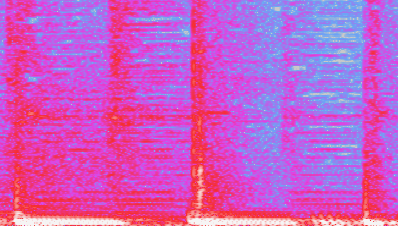
\includegraphics[width=0.47\textwidth]{\pwd/figs/spectrogram}}
	\caption{Example of a natural image and a spectrogram.}\label{fig:cat-vs-spectrogram}
\end{figure}